\chapter{SIRE et LELA}\label{ch:sire-et-lela}

Les problématiques mises en jeu par l'énergie solaire sont nombreuses.
On peut notamment citer l'intermittence, le rendement, l'approvisionnement et l'intégration des technologies associées à leur environnement, ce dernier sujet étant non trivial.
En effet, l'énergie solaire diffère des modes de production centralisés \textit{(comme les centrales thermiques ou nucléaires)} en ce qu'elle est opérée au plus près des populations, à des échelles de production plus faibles.

Il n'est alors pas rare de rencontrer des panneaux photovoltaïques dans la vie quotidienne : parkings, établissements publics et privés et habitations.
Ceci suppose un travail particulier pour l'intégration architecturale et urbanistique d'une part et l'insertion de cette production au réseau énergétique et son éventuel stockage d'autre part, en tenant compte de son caractère intermittent.

Pour traiter ces problématiques, le \gls{DTS} dispose d'un service expert sur ces domaines : le \gls{SIRE}, dont l'organigramme est présenté sur la figure \ref{fig:organigramme-DTS}.
\begin{figure}[H]
    \centering
    % Le contenu du diagramme est défini dans le fichier suivant
    \fbox{\begin{tikzpicture}[
    main/.style={text centered, text width=8cm, fill=green!20, draw, rectangle, rounded corners, font=\bfseries\Large},
    service/.style={text centered, text width=3cm, fill=gray!50, draw, rectangle, rounded corners},
    labo/.style={grow=down, xshift=4cm, text centered, text width=5cm, draw, rectangle, rounded corners, edge from parent path={(\tikzparentnode.225) |- (\tikzchildnode.west)}},
    first/.style    ={level distance=15ex},
    second/.style   ={level distance=30ex},
    third/.style    ={level distance=45ex},
    fourth/.style   ={level distance=60ex},
    fifth/.style    ={level distance=75ex},
    level 1/.style={sibling distance=12.5em, level distance=8em}]

    \node[main, anchor=south]{Département des Technologies Solaires}
    [edge from parent fork down]
    %
    child{node (d1) [service] {\textbf Service \\ Procédés \\ et \textbf Cellules \textbf Photo\textbf{v}oltaïques}}
    %
    child{node (d2) [service] {\textbf Service \textbf Modules \\ et \textbf Systèmes \textbf Photovoltaïques}
        child[labo,first]  {node {\textbf Laboratoire \\ de \textbf Stockage \textbf Stationnaire \\pour \textbf Applications ENR}}
        child[labo,second] {node {\textbf Laboratoire \\ d'\textbf Intégration \textbf Énergétique Locale \\et \textbf Autoconsommation}}
        child[labo,third]  {node {\textbf Laboratoire \\ de Pilotage \textbf Intelligent \\ des \textbf Réseaux \textbf Électriques}}
    }
    %
    child{node (d3) [service] {\textbf Service \\ \textbf Modules \\ \textbf Systèmes \textbf Photovoltaïques}};
\end{tikzpicture}}
    \caption{Organigramme simplifié de la DTS et du SIRE}
    \label{fig:organigramme-DTS}
\end{figure}

\newpage Au sein du \gls{SIRE}, le \gls{LELA} travaille spécifiquement sur la consommation énergétique des bâtiments.
À cet égard, ses enjeux scientifiques comprennent le pilotage intelligent des bâtiments et notamment la flexibilité, c'est-à-dire la possibilité de décaler les pics de consommation énergétique sur les pics de production et réciproquement.
Dans une moindre mesure, la rénovation énergétique des bâtiments est abordée par certains projets du laboratoire.

Le LELA poursuit ainsi l'objectif d'apporter une vision prospective sur les conséquences de l'équipement de bâtiments en panneaux solaires et définir des méthodologies relatives à l'adaptation de la consommation
énergétique des bâtiments, en prenant en compte différents types d’enveloppe, d'occupation et d'équipements, pour intégrer de façon prévisible et stratégique la production photovoltaïque décentralisée au réseau énergétique, passant ou non par un système de stockage intermédiaire.

Son activité est donc représentative du \gls{CEA} : les échelles des parcs de bâtiments étudiés sont locales \textit{(quartier Cambridge à Grenoble, étudié dans le cadre de cette alternance)}, nationales, européennes et mondiales\footnote{ces derniers projets, encore en cours, n'étant pas mentionnés ici pour des raisons de confidentialité}.

La trentaine de membres du laboratoire \textit{(ingénieurs chercheurs, techniciens et doctorants)} s'appuie sur des simulations numériques et sur des expérimentations à échelle réelle,
en particulier par l'utilisation active d'une des trois plateformes d'équipements de l'\gls{INES} comprenant les maisons dites "\gls{INCAS}", montrées sur la figure \ref{fig:incas},
inhabitées car spécialement dédiées aux travaux de recherche en énergétique du bâtiment.

Ces maisons sont équipées de systèmes d'instrumentation destinés à la collecte de données réelles de températures interne, externe et rayonnante, de vitesse du vent et d'humidité.
Pour fournir un caractère plus réaliste à ces données, les chercheurs attribuent une occupation type simulée.
Celle-ci se matérialise par des radiateurs placés à l'intérieur des maisons, pour représenter entre autres les déperditions de chaleur du corps humain, l'utilisation de l'eau chaude sanitaire par des valves intelligentes, l'activation programmée du chauffage et celle de la ventilation.
Les contrôles rigoureux et automatisés menés dans ces bâtiments permettent de créer une base de données réelles, fiables et exploitables.

\begin{figure}[H]
    \centering
        \subfloat[Vue extérieure \textit{(Crédit photo : Patrick Avavian)}]{\fbox{
            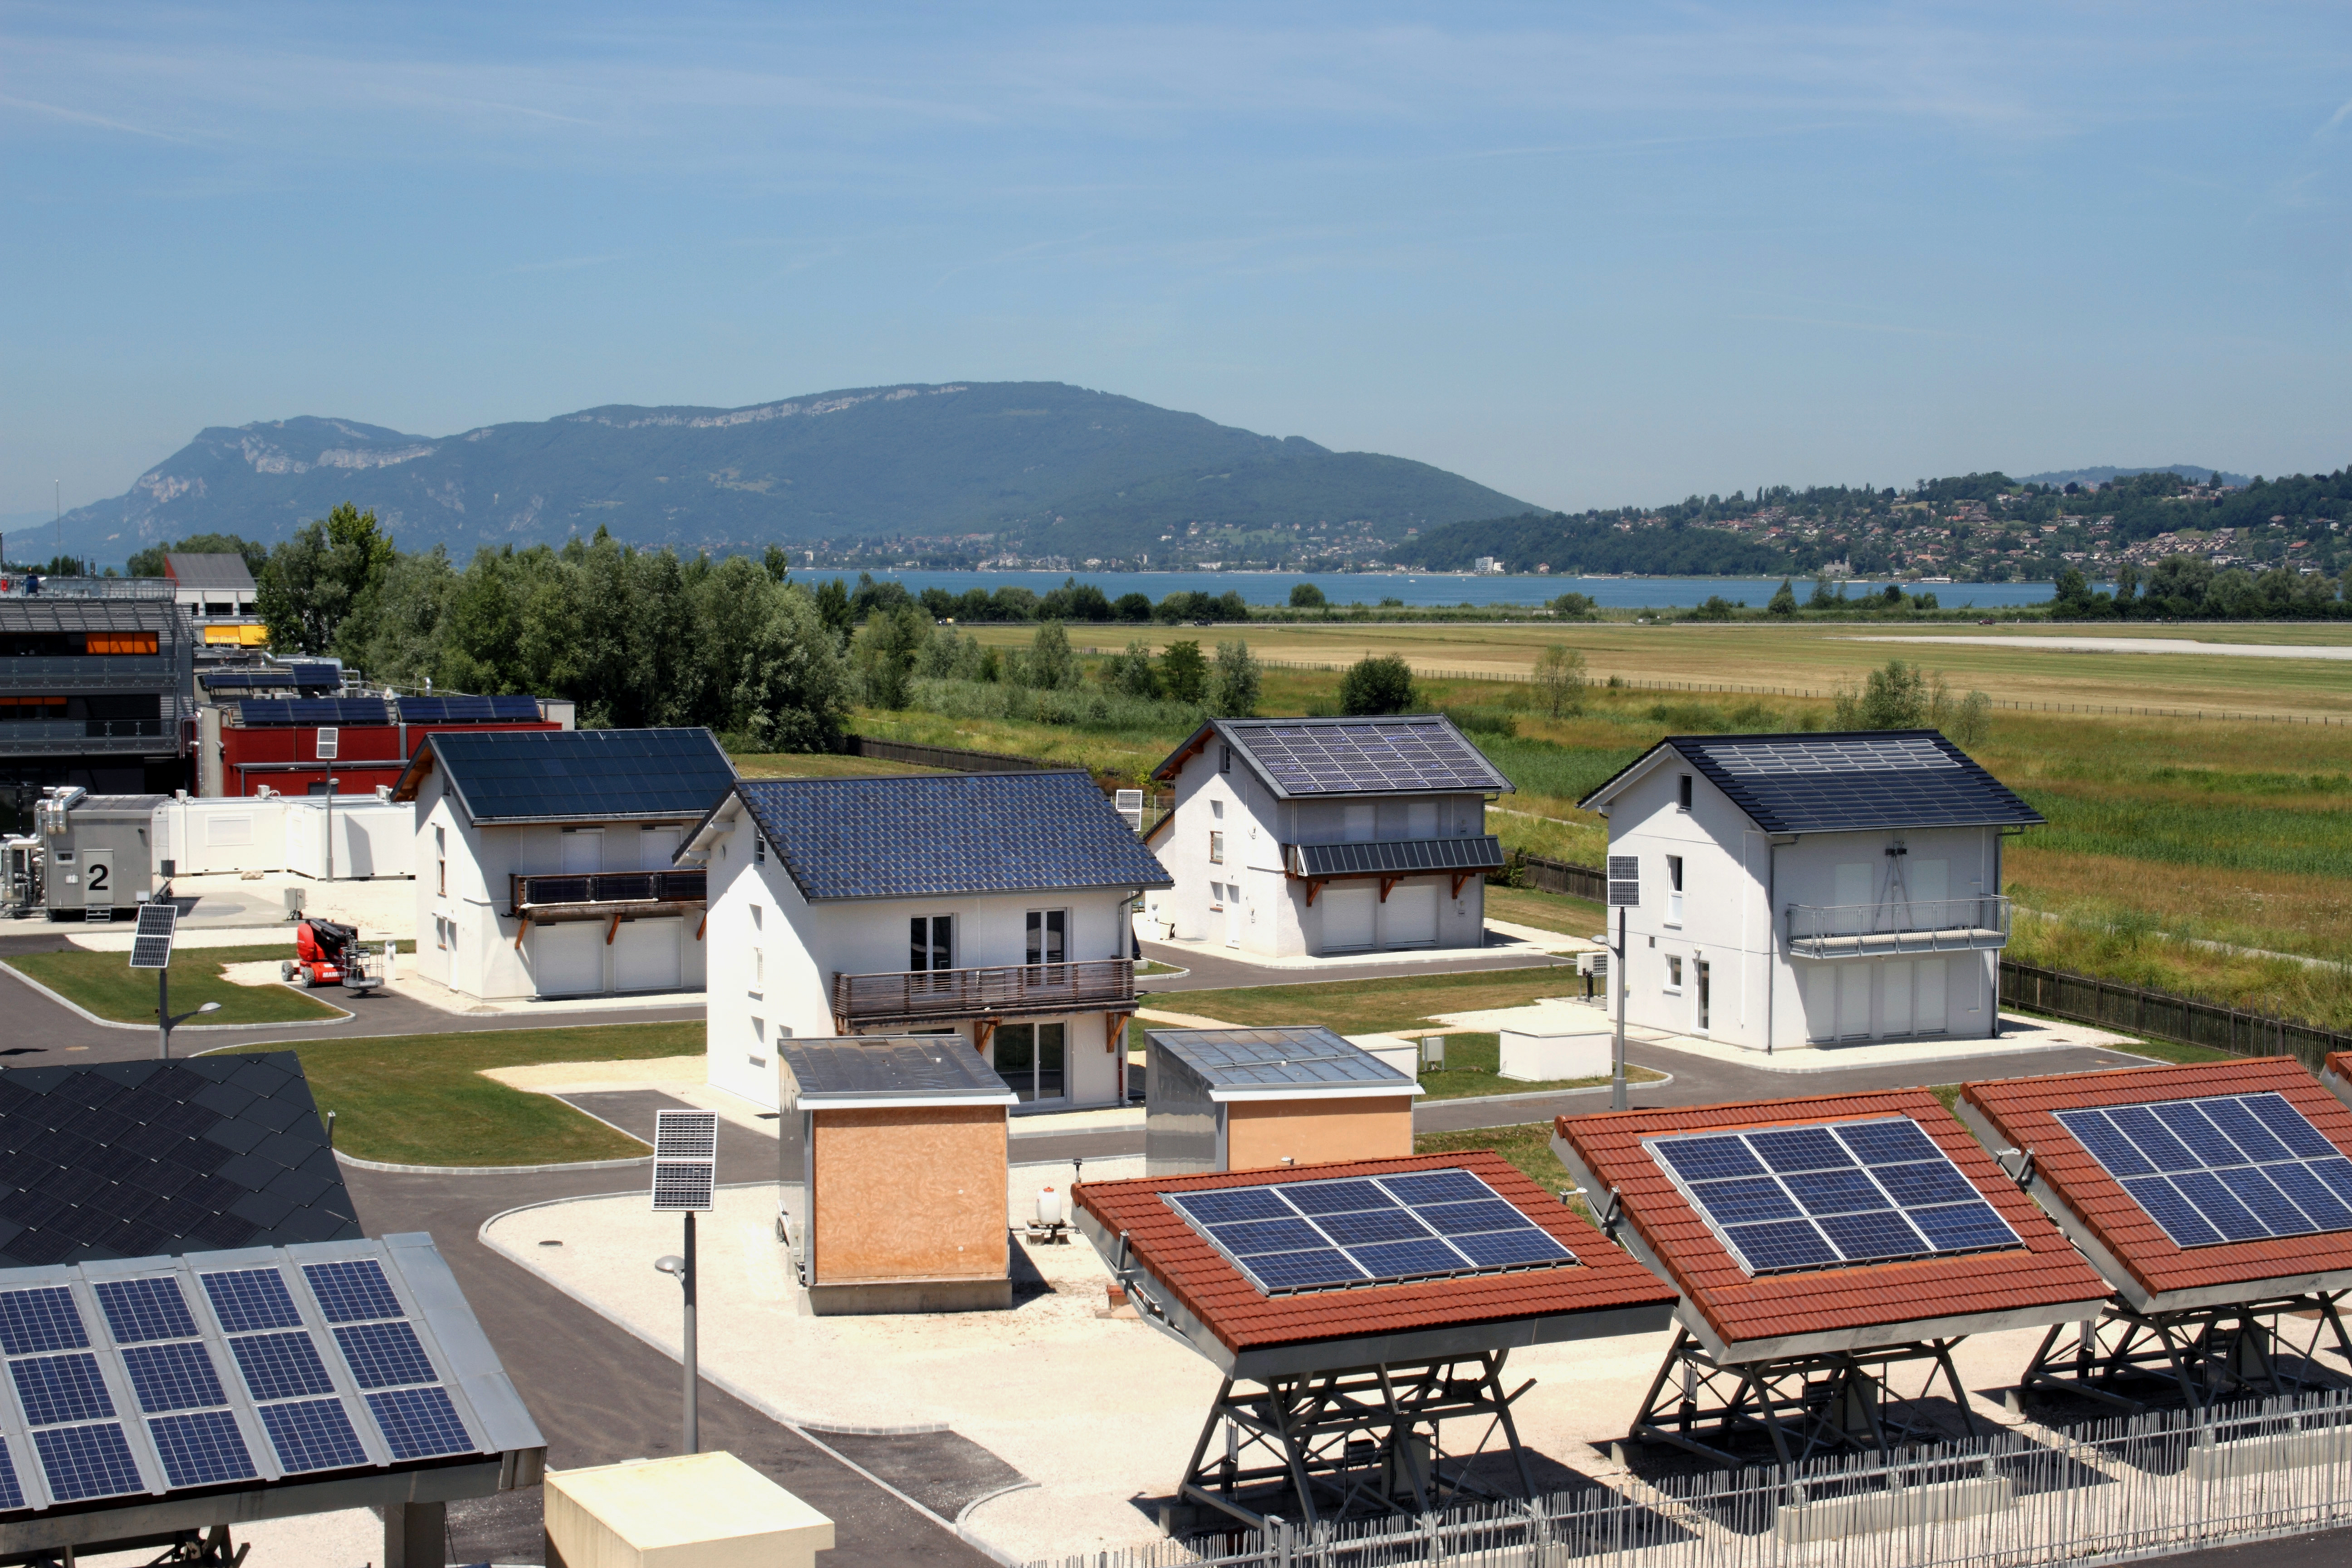
\includegraphics[width = 0.75\textwidth]{figures/illustrations/photos/INCA_Patrick AVAVIAN}}}\\
        \subfloat[Capteurs installés pour mesurer les fuites d'air vers l'extérieur \textit{(Crédit photo : Gilles Rolles)}]{\fbox{
            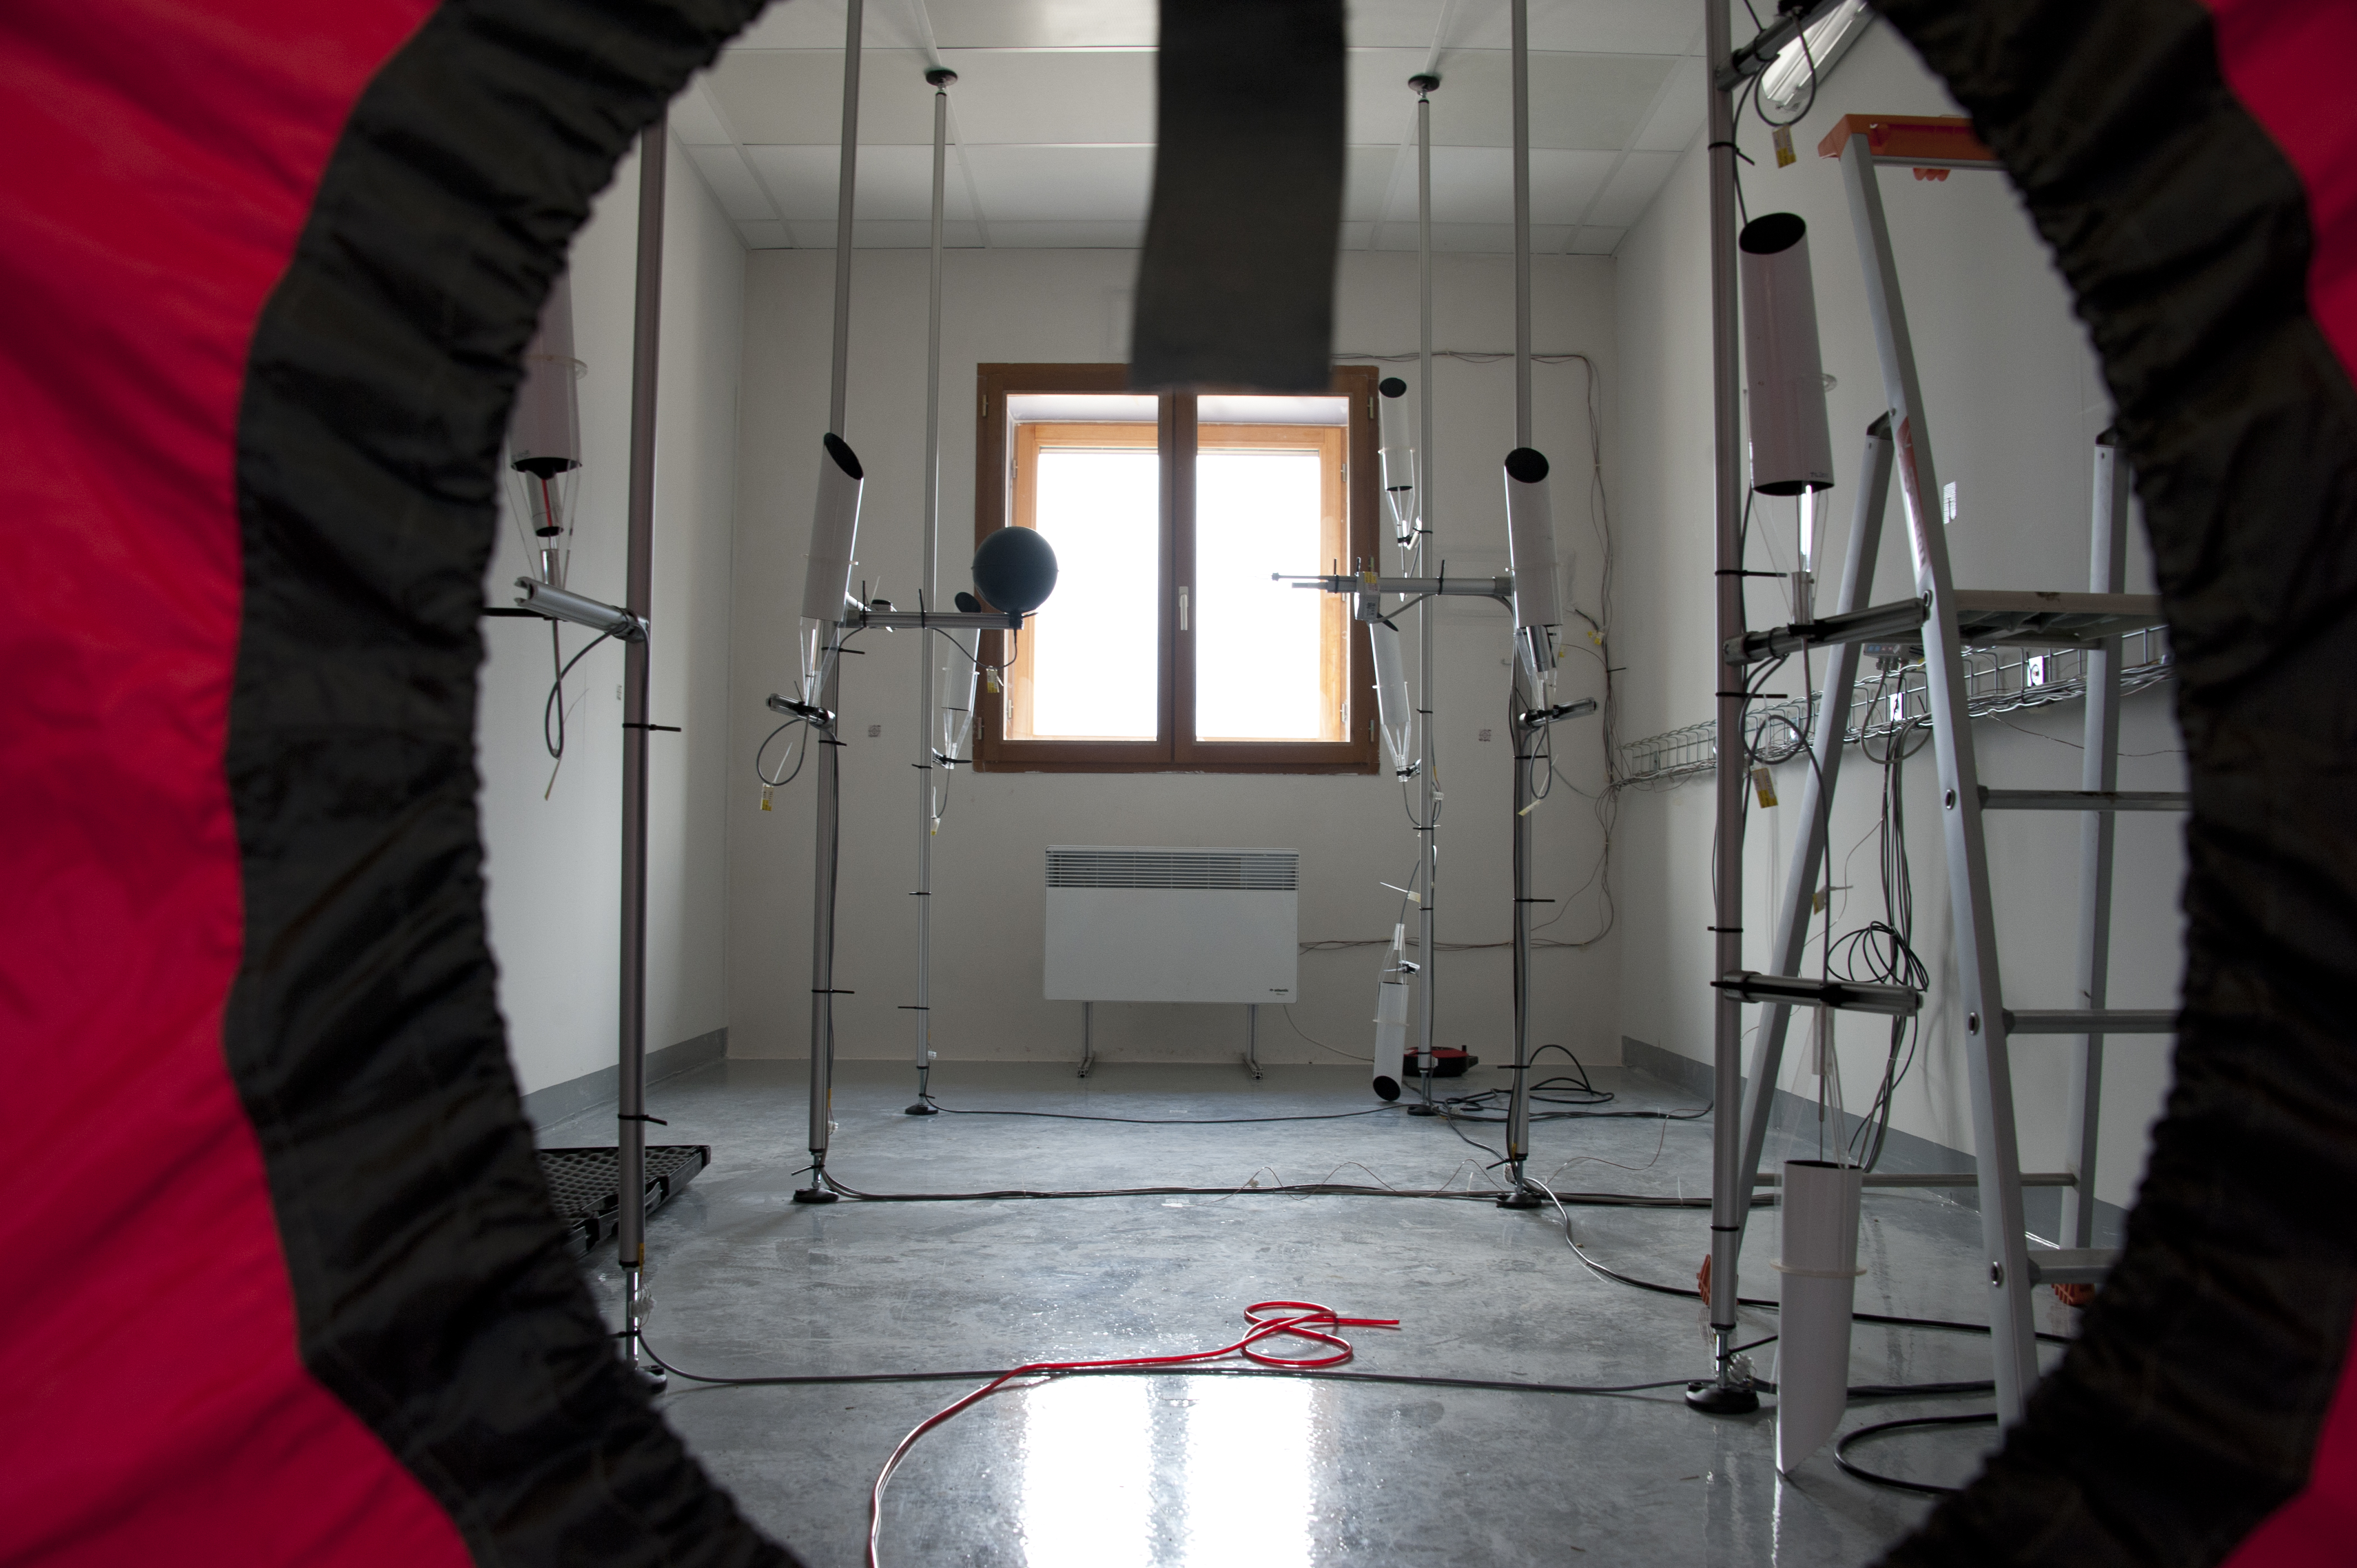
\includegraphics[width = 0.75\textwidth]{figures/illustrations/photos/INCA_int_Gilles_ROLLES}}}
    \caption{Maisons INCAS du LELA}\label{fig:incas}
\end{figure}
